% Kvarven commentary
\documentclass[12pt]{article}
\usepackage[left=2cm, right=2cm, top=2cm]{geometry}
\usepackage{graphicx}
\usepackage{hyperref}
\usepackage{wrapfig}

\usepackage[font=footnotesize, labelfont=bf]{caption}

\title{\normalsize The puzzling relationship between multi-lab replications and 
meta-analyses of the rest of the literature}
\author{\normalsize  Molly Lewis, Maya B. Mathur, Tyler J. VanderWeele, and Michael C. Frank}
\date{}

\begin{document} 
%\maketitle

\vfill 
%{\noindent Address all correspondence to Molly  Lewis,  E-mail: mollyllewis@gmail.com.\par}
\clearpage
\setcounter{page}{1}
\newpage


\begin{center} 
{\bf The puzzling relationship between multi-lab replications\\ and
meta-analyses of the rest of the literature}\\
Molly Lewis, Maya B. Mathur, Tyler J. VanderWeele, and Michael C. Frank
\end{center}

\vspace{1\baselineskip}

What is the best way to estimate the size of important effects --- should we aggregate across disparate findings using statistical meta-analysis, or instead run large, multi-lab replications (MLR)? A recent paper by Kvarven, Strømland, and Johannesson (1) compared effect size 
estimates derived from these two different methods for 15 different psychological phenomena. The authors report that, for the same phenomenon, the meta-analytic estimate tends to be about three times larger than the MLR estimate. These results pose an important puzzle: what is the relationship between these two estimates? Kvarven et al.\ suggest that their results undermine the value of meta-analysis. In contrast, in this commentary, we argue that both meta-analysis and MLR are informative but that the relationship between them is an important puzzle for future meta-research. 

Although Kvarven et al.\ show that meta-analysis and MLR produce divergent estimates of effect size, there is nevertheless a strong relationship between the two. Phenomena with larger meta-analytic estimates tend to also have larger estimates in the MLR (Pearson’s $r$ = 0.72 [0.32, 0.90], $p$ = 0.003; Fig.\ 1). Thus, although meta-analyses do show larger effects, they are not uninformative regarding the results of MLR. 

Further, many of the meta-analyses in Kvarven et al.’s study showed considerable effect heterogeneity. When effects are heterogeneous, a comparison of the meta-analytic mean to the MLR mean does not, on its own, adequately characterize the evidence for a true difference between the two. Sometimes heterogeneity can create a false impression of conflict between results when in fact differences are plausibly due to sampling variation (2). To test this idea, we examined where the MLR mean would fall in the distribution of true population effects in the meta-analysis. A median, across meta-analyses, of 20\% of the meta-analytic effect distribution was at least as small as the MLR mean estimate (Fig.\ 2, right-hand side), suggesting that many of the MLR estimates were not far outside of the meta-analytic distribution (even if they were generally smaller).

Although the discrepancy between meta-analysis and MLR results is perhaps smaller than Kvarven et al.\ suggest, a discrepancy does still exist. Effect heterogeneity alone does not account for the differences. What is the source of this discrepancy? Kvarven et al.\ speculate that it is likely due to “questionable research practices” (3) such as post-hoc analytic decision-making or publication bias. Both of these practices act as filters that select for statistically significant findings, leading to an inflation of effect size. Could these mechanisms be fully responsible? 

To test this hypothesis, we used a sensitivity analysis to estimate the meta-analytic mean under a hypothetical “worst-case” publication bias scenario (4) in which statistically significant positive studies are infinitely more likely to be published than nonsignificant and/or negative studies. To do so, we meta-analyzed  only the nonsignificant and/or negative studies, which amounts to counteracting a worst-case publication process that favors significant positive studies infinitely more than nonsignificant and/or negative studies (see SI). We analyzed the 13 of 15 meta-analyses for which the meta-analytic mean estimate was larger than the MLR estimate and for which these analyses were statistically estimable (meta-analyses must contain at least one study that is not significant or has a negative effect size). For the majority of these (62\%), even worst-case publication bias of this nature could not attenuate the meta-analytic estimate to match that of the MLR. Also, for all but one of these meta-analyses (i.e. 92\%), worst-case publication bias could not attenuate the meta-analytic estimate all the way to the null (Fig.\ 2). It therefore appears somewhat implausible that a realistic mechanism of publication bias, no matter how severe, could entirely explain the discrepancy between meta-analytic and MLR effect size estimates.

What, then, are other possible causes of the discrepancy? One possibility is that the phenomena being studied may be sensitive to the details of the experimental materials and methods, and especially to how these interact with the specific populations being assessed. While this kind of method- and context-sensitivity has frequently been cited as a specifically post-hoc explanation for direct replication failures (5), a series of pre-registered replications that we and our collaborators have carried out attest to the importance of small methodological factors in reproducing effects (6-8). 

Investigators who are committed to understanding a particular phenomenon may take pains to tailor their stimuli to a particular context. Perhaps this is one reason that the individual studies in a meta-analysis typically vary considerably in their methods and stimuli. In contrast, MLRs typically standardize their materials across all populations and contexts being studied in order to establish a single method for all participating labs. This difference could account for some of the discrepancy in effect sizes. For example, one of the phenomena included in Kvarven et al.’s paper is an effect whereby imagining interaction with an outgroup member leads participants to be more likely to express an intention to engage with an outgroup member in real life. In the original paper (9), the participants were British non-Muslim undergraduates, and the “outgroup” was British Muslims. In the corresponding MLR, 34 out of the 35 replication sites used the same outgroup, “Muslim,” despite the fact that the sites spanned nine different countries with likely varying degrees of prejudice toward Muslims. In contrast, in the meta-analysis, individual studies used a wide range of outgroups, adapted to the local social context of each study. Furthermore, even if labs were to likewise alter the stimuli according to context, individual studies may be more likely than MLR's to select samples and exclusion criteria to maximize effect sizes.

More broadly, in social psychology, effects may be more context sensitive relative to other psychological domains (5,10). Notably, the majority of phenomena in the target paper concern effects that appear social or contextually-dependent (e.g., interactions between political belief and moral decision-making, humor responses, imagined intergroup contact, expression of prejudice). To carry empirical weight, such speculations must be tested directly in future meta-scientific work. 

Yet another source of the discrepancy may be that in individual studies, as compared with MLRs, investigators, feeling that more is at stake, may make greater effort to ensure intervention fidelity, thereby increasing effect sizes. This is not investigator bias; this is that the intervention itself is effectively different (e.g. greater encouragement to engage).

In summary, both meta-analysis and MLRs provide methods for estimating the effect size of important phenomena by aggregating evidence across multiple studies. Kvarven et al.\ present the first systematic comparison of these two methods and show that effect sizes derived from meta-analyses are puzzlingly larger than those derived from MLRs. Our analyses suggest that effect size heterogeneity and publication bias may contribute but are unlikely to account fully for this discrepancy. Speculative possibilities for the remaining discrepancy include that MLRs obtain smaller effect sizes because of standardization of methods across labs for phenomena that are context-sensitive and because of potential differential effort to ensure intervention fidelity. Understanding the source of the discrepancy between the two methods is an important, complex question for future meta-scientific research.

\pagebreak

\begin{figure}[h!]
\centering
     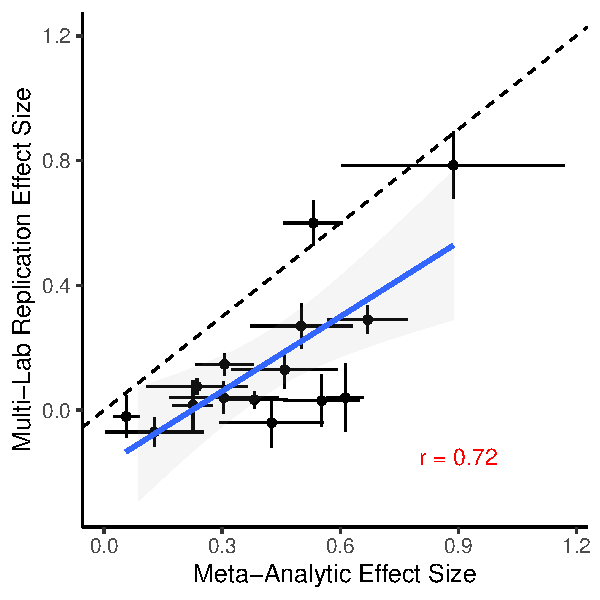
\includegraphics[width=5in]{../results/analysis_1/fig1a.pdf}
      \caption{  Correlation between effect size estimates from multiple-laboratory replications and random effect meta-analytic estimates (Pearson’s $r$(13) = 0.72 [0.32, 0.9], $p$ = 0.003). Each point corresponds to a phenomenon ($N$ = 15), and ranges indicate 95\% confidence intervals. The dashed reference line has a slope of 1. }
\end{figure}

\begin{figure}[h!]
\centering
     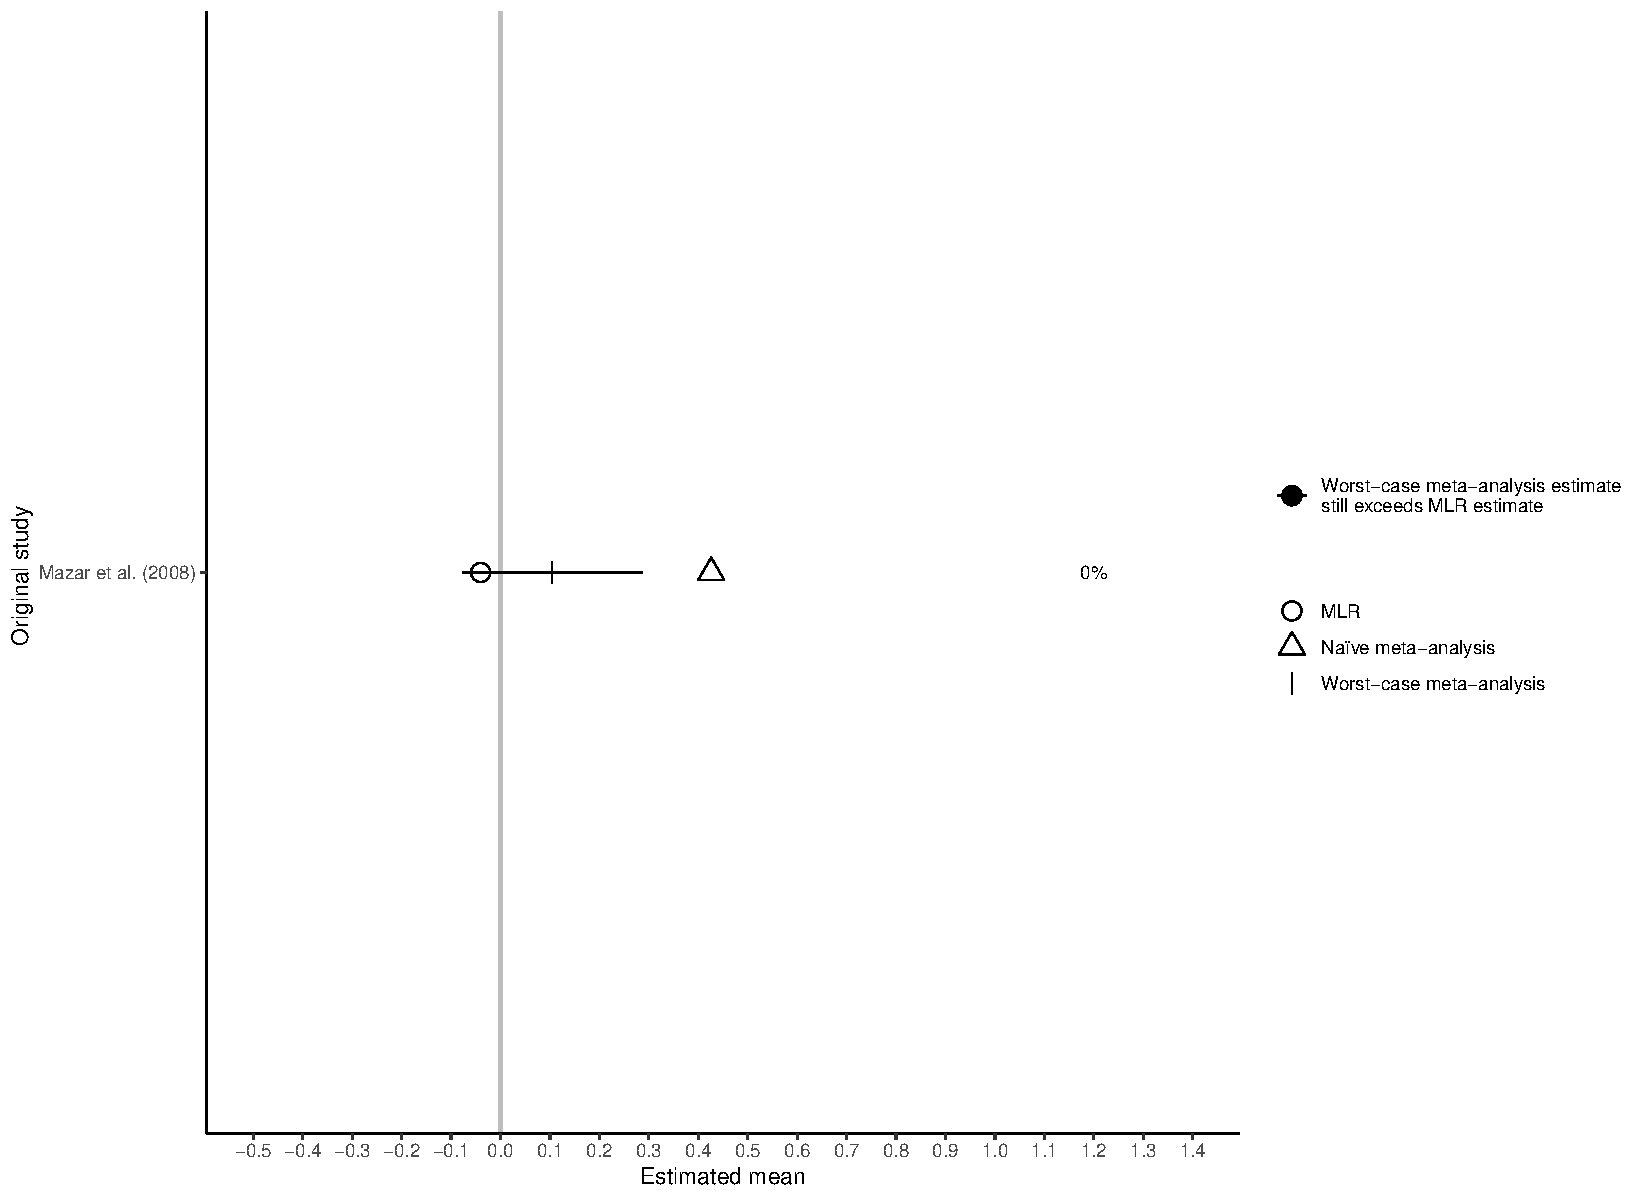
\includegraphics[width=7in]{../results/analysis_2/forest.pdf}
      \caption{Estimates from sensitivity analyses representing worst-case publication bias (vertical tick marks with 95\% confidence intervals [CI]) versus naïve meta-analysis estimates (diamonds) and multi-lab replication estimates (MLR; circles). Meta-analyses are ordered by their naïve estimates. For orange-colored meta-analyses, the worst-case estimate exceeds the MLR estimate, indicating that no amount of publication bias that purely favors statistically “significant” and positive results could entirely explain the discrepancy between the naïve estimate and the MLR estimate. Percentages and 95\% CIs on the right-hand side represent the estimated percentage of true population effects in the naïve meta-analysis that are as small as, or smaller than, the MLR estimate. CIs are omitted when they were not estimable via bias-corrected and accelerated bootstrapping (11).}
\end{figure}
\pagebreak


\subsubsection*{Code availability}
The analysis code for all analyses is available at the project’s Github repository (link: \url{https://github.com/mllewis/kvarven_reanalysis}).


\subsubsection*{References}

1. Kvarven, A., Strømland, E., \& Johannesson, M. Comparing meta-analyses and preregistered multiple-laboratory replication projects. {\it Nature Human Behaviour}, 1-12 (2019)
 \vspace{3mm}
 
\noindent2. Mathur, M. B., \& VanderWeele, T. J. (2019). Finding common ground in meta-analysis “wars” on violent video games. {\it  Perspectives on Psychological Science,} 14(4), 705-708.
\vspace{3mm}

\noindent3. EJ Masicampo and Daniel R Lalande. A peculiar prevalence of p values just below .05. {\it The Quarterly Journal of Experimental Psychology}, 65(11):2271–2279, 2012.433
\vspace{3mm}

\noindent4. Mathur, M. B., \& VanderWeele, T. J. (under review). Sensitivity analysis for publication bias in meta-analyses. Preprint retrieved from:  \url{ https://osf.io/s9dp6/}.
\vspace{3mm}

\noindent5. Van Bavel, J. J., Mende-Siedlecki, P., Brady, W. J., \& Reinero, D. A. (2016). Contextual sensitivity in scientific reproducibility.  {\it Proceedings of the National Academy of Sciences}, 113(23), 6454-6459.
\vspace{3mm}

\noindent6. Phillips, J., Ong, D. C., Surtees, A. D., Xin, Y., Williams, S., Saxe, R., \& Frank, M. C. (2015). A second look at automatic theory of mind: Reconsidering Kovács, Téglás, and Endress (2010).  {\it Psychological Science}, 26(9), 1353-1367.
\vspace{3mm}

\noindent7. Lewis, M. \& Frank, M. C. (2016). Understanding the effect of social context on learning: A replication of Xu and Tenenbaum (2007b).  {\it Journal of Experimental Psychology: General}, 145(9), e72– e80.
\vspace{3mm}

\noindent8. Lewis, M. L. \& Frank, M. C. (2018). Still suspicious: The suspicious-coincidence effect revisited.  {\it Psychological Science}, 29(12), 2039-2047.
\vspace{3mm}

\noindent9. Husnu, S. \& Crisp, R. J. Elaboration enhances the imagined contact effect. {\it Journal of Experimental Social Psychology} 46, 943-950 (2010).
\vspace{3mm}

\noindent10. Inbar, Y. (2016). Association between contextual dependence and replicability in psychology may be spurious.  {\it Proceedings of the National Academy of Sciences}, 113(34), E4933-E4934.
\vspace{3mm}

\noindent11.  Mathur, M. B., \& VanderWeele, T. J. (in press). Robust metrics and sensitivity analyses for meta-analyses of heterogeneous effects. {\it Epidemiology}.


\subsubsection*{Acknowledgments}
Eirik Strømland provided forthcoming answers to our questions about his paper. We thank Martin Hagger for a thought-provoking discussion. 	

\subsubsection*{Author contributions}
M.L. and M.B.M. conducted the analyses. All authors wrote the paper.

\subsubsection*{Competing information}
The authors declare no competing interests.


\end{document}
